\begin{tikzpicture} [scale = 1.5]
  \draw[black] (0, 0) grid [xstep = 2, ystep = 2] (4.2, -4.2);

  \foreach \i in {0, 2, 4}
    \foreach \j in {0, -2, -4}
      \node[shape = circle, fill = blue] at (\i, \j) {};


  \foreach \i in {1, 3}
    \foreach \j in {-1, -3}
      \node[shape = circle, draw = blue, thick] at (\i, \j) {};

  \foreach \i in {1, 3}
    \foreach \j in {0, -2 ,-4}
      \node[shape = rectangle, fill = red] at (\i, \j) {};

  \foreach \i in {0, 2, 4}
    \foreach \j in {-1, -3}
      \node[shape = rectangle, fill = green] at (\i, \j) {};

  \node[shape = circle, fill = blue] at (5, -0.5) {};
  \node[right = 5pt] at (5, -0.5) {$v_x, \nicefrac{1}{\rho}$};
  \node[shape = circle, draw = blue, thick] at (5, -1.5) {};
  \node[right = 5pt] at (5, -1.5) {$v_z, \nicefrac{1}{\rho}$};
  \node[shape = rectangle, fill = red] at (5, -2.5) {};
  \node[right = 5pt] at (5, -2.5) {$\tau_{xx}, \tau_{zz}, (\lambda + 2\mu), \lambda$};
  \node[shape = rectangle, fill = green] at (5, -3.5) {};
  \node[right = 5pt] at (5, -3.5) {$\tau_{xz}, \mu$};

  \node[above = 12pt] at (0, 0) {$i - 1$};
  \node[above = 12pt] at (2, 0) {$i$};
  \node[above = 12pt] at (4, 0) {$i + 1$};
  \node[above = 12pt] at (3, 0) {$i'$};

  \node[left = 12pt] at (0, 0) {$j - 1$};
  \node[left = 12pt] at (0, -2) {$j$};
  \node[left = 12pt] at (0, -4) {$j + 1$};
  \node[left = 12pt] at (0, -3) {$j'$};

\end{tikzpicture}
